\documentclass[a4paper,norsk, 10pt]{article}
\usepackage[utf8]{inputenc}
\usepackage{verbatim}
\usepackage{listings}
\usepackage{graphicx}
\usepackage[norsk]{babel}
\usepackage{a4wide}
\usepackage{color}
\usepackage{amsmath}
\usepackage{float}
\usepackage{amssymb}
\usepackage[dvips]{epsfig}
\usepackage[toc,page]{appendix}
\usepackage[T1]{fontenc}
\usepackage{cite} % [2,3,4] --> [2--4]
\usepackage{shadow}
\usepackage{hyperref}
\usepackage{titling}
\usepackage{marvosym }
%\usepackage{subcaption}
\usepackage{subfig}
\usepackage[noabbrev]{cleveref}
\usepackage{cite}
\usepackage{todonotes}


\setlength{\droptitle}{-10em}   % This is your set screw

\setcounter{tocdepth}{2}

\lstset{language=c++}
\lstset{alsolanguage=[90]Fortran}
\lstset{alsolanguage=Python}
\lstset{basicstyle=\small}
\lstset{backgroundcolor=\color{white}}
\lstset{frame=single}
\lstset{stringstyle=\ttfamily}
\lstset{keywordstyle=\color{red}\bfseries}
\lstset{commentstyle=\itshape\color{blue}}
\lstset{showspaces=false}
\lstset{showstringspaces=false}
\lstset{showtabs=false}
\lstset{breaklines}
\title{STK4900 Oblig 2}
\author{Daniel Heinesen, daniehei}
\begin{document}
\maketitle

\section{Problem 1}
\subsection{a)}
We have a data set where the outcome is whether the female crab has one or more satellites $y = 1$, or none $y=0$. We are looking for a regression that can, given the covariates, give us a probability that the female crab have satellites. This means that we are looking for a regression model that gives us a probability for a binary outcome. The best choice for such a model is a logistic regression model
\begin{equation}
p(x_1,...,x_p) = \frac{\exp(\beta_0 + \beta_1 x_1 + ... + \beta_n x_n)}{1+\exp(\beta_0 + \beta_1 x_1 + ... + \beta_n x_n)},
\end{equation}
where $p$ is the desired probability, $x_i$ the covariates and $\beta_i$ their fitted coefficients\todo{Is that the best way to describe  $\beta_i$?}.

\subsection{b)}

We want to find the odds ratio between crabs that differ with one centimetre in with. We know that with width as the only covariate, we define the odds as 

\begin{equation}
\frac{p(x)}{1-p(x)} = \exp(\beta_0 + \beta_1 x).
\end{equation}
From this we get the odds ratio for a difference in one centimetre
\begin{equation}
OR = \frac{p(x+1)/[1-p(x+1)]}{p(x)/[1-p(x)]} = \frac{\exp(\beta_0 + \beta_1\cdot (x+1))}{\exp(\beta_0 + \beta_1 x)} = \exp(\beta_1\cdot 1) = \exp(\beta_1).
\end{equation}


\begin{table}[!ht]
\centering
\begin{tabular}{rrrrr}
  \hline
 & Estimate & Std. Error & z value & Pr($>$|$z$|) \\ 
  \hline
(Intercept) & -12.3508 & 2.6287 & -4.70 & 0.0000 \\ 
  width & 0.4972 & 0.1017 & 4.89 & 0.0000 \\ 
   \hline
\end{tabular}
\caption{Summary of the logical regression done the satellite crabs, with width as the only covariate.}\label{tab:crab_width}
\end{table}

We get the $\beta$'s from the logical regression found in table \ref{tab:crab_width}. From this we see that 
\begin{equation}
OR = \exp(0.4972) = 1.64.
\end{equation}
This means that odds of a female crab having satellite males increase by $64\%$ if the width of female increases by $1$ cm.

If $p(1) = p(x+1)$ and $p(0)=p(x)$ are small, we can approximate the odds ratio with the relative risk $RR = p(1)/p(0)$. In this case we have that $p(1) = 6.8\cdot 10^{-6}$ and $p(0) = 4.1 \cdot 10^{-6}$, which means that both are very small. This means that we can assume that $RR \approx OR$. And comparing them $OR = 1.6367$ and $RR = 1.6487$ we see that this is correct.

Since we know that 
\begin{equation}
t = \frac{\beta}{se(\beta)}
\end{equation}
is close to normally distributed, we can use this to find a confidence interval for the odds ratio. We simply do this by calculating the confidence interval for $\beta_1$ and then taking $\exp$ of this interval. 

\begin{table}[!ht]
\centering
\begin{tabular}{rrrr}
  \hline
 & expcoef & lower & upper \\ 
  \hline
(Intercept) & 4.33e-06 & 2.50-08 & 0.00075 \\ 
  width & 1.64 & 1.35 & 2.01 \\ 
   \hline
\end{tabular}
\caption{Confidence interval for the odds ratio for crabs differing by one cm in width.}\label{tab:crabs_OR_CI}
\end{table}

From tab. \ref{tab:crabs_OR_CI} we see that we get a confidence interval $CI = (1.35,2.01)$. Since $1$ is outside of this interval, we can say that width gives an significant increase in the probability of satellites. 

\subsection{c)}

\subsection{d)}
\subsection{e)}


\section{Problem 2}
\subsection{a)}
We have an outcome, medals, which is a count outcome, and we therefore assume that the count is distributed with a Poisson distribution $Y_i \sim Po(\lambda_i)$. Such a distribution is parametrized with a parameter $\lambda$, the rate. In our data we will have that this rate is dependent on several covariates, so we need a way to determine this dependence on the covariates. It is here we use Poisson regression. Given $n$ independent subjects, we have that 
\begin{itemize}
\item $y_i$ is the count of the $i^{th}$ subject
\item $x_{ij}$ is the $j^{th}$ covariate for the $i^{th}$ subject
\end{itemize}
We then define our model as 
\begin{equation}
\lambda_i = \lambda(x_{1,i},...,x_{p,i}) = \exp(\beta_0 + \beta_1 x_{1,i} + ... + \beta x_{p,i}).
\end{equation}

It is this model we want to fit to the medal counts. But there is something we have to be careful with: A country with a higher number of athletes will most likely have more medals than a country with fewer athletes. So instead of the medal count following the distribution $Y_i ~ Po(\lambda_i)$ we instead say that they follow the distribution $Y_i ~ Po(w_i\lambda_i)$, where $w_i$ is the number of athletes representing the country. But how do use this in our model? We can see this from taking the expected value

\begin{equation}
E[Y_i] = w_i \lambda_i = w_i\exp(\beta_0 + \beta_1 x_{1,i} + ... + \beta x_{p,i}) = \exp(\log(w_i) + \beta_0 + \beta_1 x_{1,i} + ... + \beta x_{p,i}).
\end{equation}

This means that to compensate for this imbalance of athletes, we can fit out model with $\log(w_i)$ as a covariate. This is what we call an offset. This we already $Log.athletes$ in our data, we can just use this as the offset in our regression.

\subsection{b)}
To find a fit for our model we are going to use two methods. The first is to fit a model with all the covariate and see which of them are significant. The other method is to add one covariate after an other and use a two-way ANOVA to see if the addition is significant.

\begin{table}[!htb]
\centering
\begin{tabular}{rrrrr}
  \hline
 & Estimate & Std. Error & z value & Pr($>$|$z$|) \\ 
  \hline
(Intercept) & -2.8623 & 0.3191 & -8.97 & 0.0000 \\ 
  Log.population & 0.0275 & 0.0315 & 0.87 & 0.3831 \\ 
  GDP.per.cap & -0.0149 & 0.0032 & -4.65 & 0.0000 \\ 
  Total1996 & 0.0118 & 0.0016 & 7.36 & 0.0000 \\ 
   \hline
\end{tabular}
\caption{Summary of a Poisson regression with all the covariates. $Log.popilation$ is the logarithm of the nation's population size per 1000, $GDP.per.cap$ is the GDP per capita and $Total1996$ is the medal count for the previous Olympic Games.}\label{tab:ol_full_it}
\end{table}


From table\ref{tab:ol_full_it} we see the summary of the fit with all covariate. We see that with p-values close to $0$




\section{Problem 3}

\subsection{a)}
We are here looking at the survival of patients with cirrhosis treated with prednisone. We are first going to look at the Kaplan-Meier plots, which are plots of the estimated survival function. We are going to look at four different plots corresponding to treatment(whether the patient got prednisone or a placebo), the sex of the patient, the severity of fluid build up in the abdomen (ascites) at the start of the observation, and their age group.

\begin{figure*}[!htbp]
\centering
\begin{tabular}{@{}ccc@{}}
\subfloat[Survival function for the different treatments. We see that there is some difference, with patients treated with the placebo having lower survival during most of the study. But the difference is very small.\label{fig:KM_treat}]{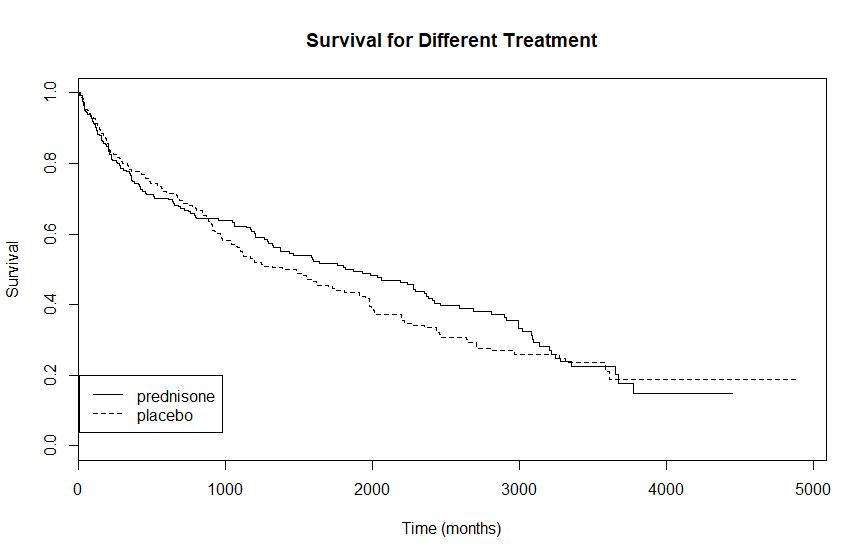
\includegraphics[width=0.5\textwidth]{KM_treat.png}} & 
\subfloat[The figure shows that the survival for male patients are smaller than that for the female patients. The difference is not large, and may not be significant.\label{fig:KM_sex}]{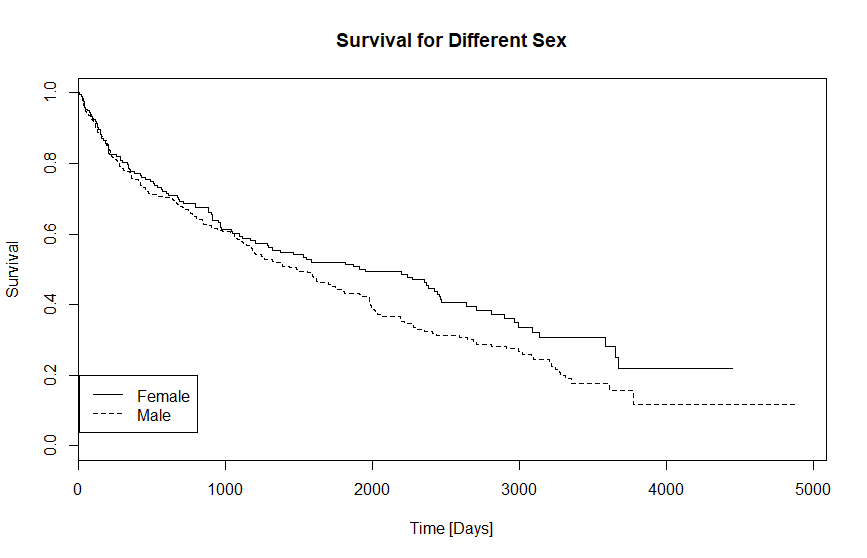
\includegraphics[width=0.5\textwidth]{KM_sex.png}} \\
\subfloat[The figure shows that there is a large difference in the survival based on the severity of the ascites of the patient at the start of the observation. The more fluid the patient has, the lower the survival.\label{fig:KM_asc}]{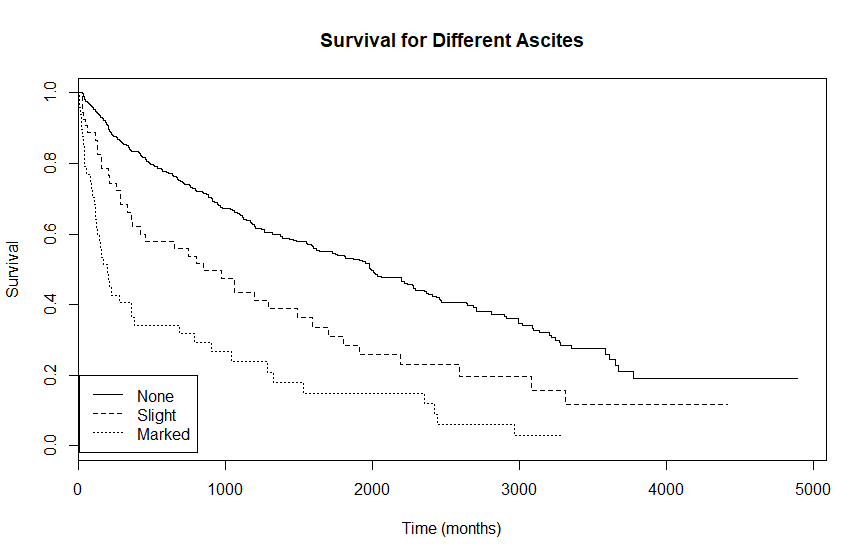
\includegraphics[width=0.5\textwidth]{KM_asc.png}} &
\subfloat[The figure shows that the age plays a important role in the survival, with older patients surviving shorter than the younger ones.\label{fig:KM_age}]{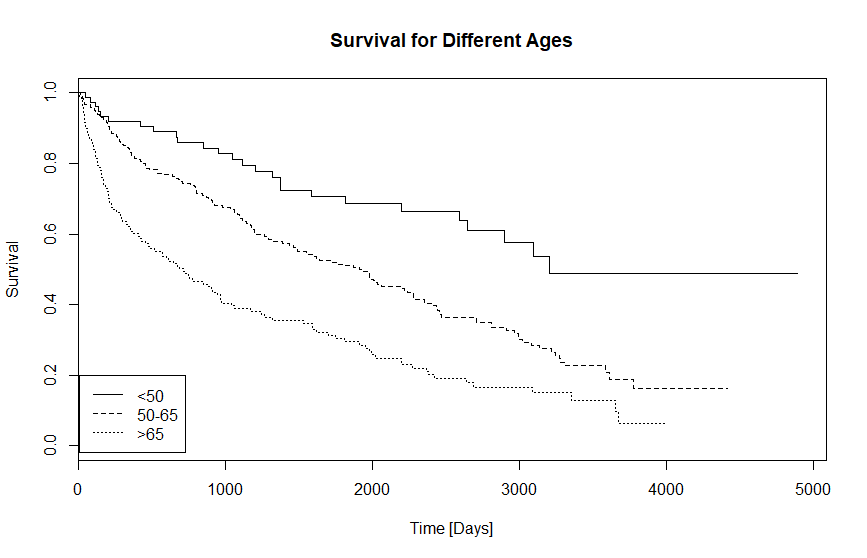
\includegraphics[width=0.5\textwidth]{KM_age.png}} 
\end{tabular}
\caption[]{Four figure showing the estimated survival function for different groups.}
\label{fig:KM}
\end{figure*}

If we look at figure \ref{fig:KM} we see the different Kaplan-Meier plots for the different groups. Fig. \ref{fig:KM_treat} shows the difference in survival based on the treatment. We see that, (especially in the middle of the observation) patients with placebo the survival seems to be lower than for the patients with prednisone. This may indicate that the treatment helps, but we see that the difference is so small that the difference may be due to other factors.

Looking at fig. \ref{fig:KM_sex} we can clearly see that male patients has a lower survival for the entire observational period than female period. But again the difference is so small that we ought to be sceptical about the significance.

For the ascites, fig. \ref{fig:KM_asc}, the difference in the severity of the fluid buildup seems to have a large impact on the survival of the patients. There is a clear decrease in survival for a patient with slight ascites compared with one with none, and an even wore decrease if the patient has marked ascites.

The same clear difference can be seen in the estimated survival of the groups with different ages, fig. \ref{fig:KM_age}. The survival of the decreases drastically with the increase in age.


\subsection{b)}

We have seen above that there is some difference in all the $K$ different groups. Now we want to check if these differences are significant. To check this we are going to use \textit{logrank tests}. In this test we test the null hypothesis that a set with groups have the same survival function. We do this by finding the observed number of events in each group, giving us $O_i$. Then we find the expected number of events $E_i$, which is the number of observations we would expect if all the groups were the same. With these we can compute the $\chi^2$ test statistic

\begin{equation}
\chi^2_i = \frac{(O_i - E_i)^2}{se(O_i-E_i)}.
\end{equation}

This follows a $\chi^2$ distribution with $K-1$ degrees of freedom.

\begin{table}[!htb]
\centering
\begin{tabular}{c|c|c|c|c|c}
Type & N & Observed & Expected & $(O-E)^2/E$ & $(O-E)^2/V$ \\
\hline 
treat=0 & $251$ & $142$ &  $149$&  $0.355$&  $0.728$ \\
treat=1 & $237$ & $150$ &  $143$&  $0.371$&  $0.728$ \\
\hline\\
Treatment & \multicolumn{5}{l}{Chisq= 0.7  on 1 degrees of freedom, p= 0.4}\\
\hline
\hline
sex=0 & $198$ & $111$ &  $127$&  $2.00$&  $3.55$ \\
sex=1 & $290$ & $181$ &  $165$&  $1.54$&  $3.55$ \\
\hline\\
Sex & \multicolumn{5}{l}{Chisq= 3.5  on 1 degrees of freedom, p= 0.06}\\
\hline
\hline
asc=0 & $386$ & $211$ &  $251.9$&  $6.63$&  $48.66$ \\
asc=1 & $54$ & $39$ &  $26.2$&  $6.30$&  $6.94$ \\
asc=2 & $48$ & $42$ &  $14.0$&  $56.7$&  $59.6$ \\
\hline\\
Ascites & \multicolumn{5}{l}{Chisq= 69.9  on 2 degrees of freedom, p= 7e-16 }\\
\hline
\hline
agegr=0 & $80$ & $26$ &  $58.7$&  $18.18$&  $22.87$ \\
agegr=1 & $250$ & $148$ &  $162.0$&  $1.21$&  $2.72$ \\
agegr=2 & $158$ & $118$ &  $71.3$&  $30.51$&  $40.87$ \\
\hline\\
Ascites & \multicolumn{5}{l}{Chisq= 50.6  on 2 degrees of freedom, p= 1e-11}\\
\end{tabular}
\caption{Table showing logrank tests for the different groups.}\label{tab:logrank}
\end{table}


Table \ref{tab:logrank} shows us the logrank tests for the different covariates with their respective groups. Looking at the difference between placebo and prednisone we see that we have a small $\chi^2 = 0.7$ and large $p=0.4$. This means that we cannot conclude that prednisone increase survival -- as we saw in fig. \ref{fig:KM_treat}.

In the difference between male and female patients, we see in fig. \ref{fig:KM_sex} there female patients seemed to have a bit longer than male patients. But from tab. \ref{tab:logrank} we see that we get a statistic $\chi^2 = 3.5$ and $p=0.006$. This means the $p$ is a bit too large for us to say that it is significant. Thus we cannot conclude that there is a difference between the sexes.

Fro both ascites and age group we saw in fig. \ref{fig:KM_asc} and \ref{fig:KM_age} that there seems to be a large difference in the survival between the groups. From tab. \ref{tab:logrank} we see for the difference severities of ascites we get $\chi^2 = 69.9$ and $p=7\cdot10^{-16}$, and for different age groups we get $\chi^2 = 50.6$ and $p=1\cdot10^{-11}$. So we conclude that there is a significant difference between the different severities in ascites, and there is a significant difference between the age groups.


\subsection{c)}
We now want to estimate the hazard function given out covariates. This is done with a Cox regression, where we estimate the hazard function as
\begin{equation}
h(t|x_1,...,x_p) = h_0(t)\exp(\beta_1 x_1 + ... + \beta_p x_p),
\end{equation}
where $h_0(t)$ is the baseline hazard function, given as the hazard when all covariates are zero.

Here we want to use Cox regression with ascites, treatment and sex as categorical covariates and age as a numerical covariate.


\begin{table}[!htb]
\centering
\begin{tabular}{rrrrrr}
  \hline
 & coef & exp(coef) & se(coef) & z & p \\ 
  \hline
factor(sex)1 & 0.46 & 1.59 & 0.13 & 3.68 & 0.000236 \\ 
  factor(treat)1 & 0.04 & 1.05 & 0.12 & 0.38 & 0.703263 \\ 
  factor(asc)1 & 0.60 & 1.83 & 0.18 & 3.45 & 0.000564 \\ 
  factor(asc)2 & 1.19 & 3.28 & 0.18 & 6.78 & 1.24e-11 \\ 
  age & 0.05 & 1.05 & 0.01 & 7.14 & 9.26e-13 \\ 
   \hline
\end{tabular}
\caption{Table showing a part of the summary of the Cox regression, with the exponent of the coefficients included.}\label{tab:cox}
\end{table}

Table \ref{tab:cox} shows the result of the Cox regression. We that once again the severity of ascites and age have significant effects on the hazard, with both increase in severity and age leading to an increase in hazard. Contrary to our logrank test, where sex did not have a significant effect on survival, we see that sex have a significant effect on the hazard, with male patients having a larger hazard.

We can find the hazard ratio for men versus women by observing that

\begin{equation}
\frac{h(t|x_1,...,x_{p-1},x_{sex} = 1 = male)}{h(t|x_1,...,x_{p-1},x_{sex} = 0 = female)} = \exp(\beta_{sex}) = \exp(0.46) = 1.59.
\end{equation}
This means that the hazard increases with $59\%$ if the patient is male. Since
\begin{equation}
t = \frac{\beta_i}{se(\beta_i)}
\end{equation}
is close to normally distributed \todo{is it?}, we can find the $95\%$ confidence interval for this hazard ratio as $\exp(\beta_i) \pm \exp(1.96\cdot se(\beta_i))$, which gives us the interval
\begin{equation}
CI = (1.241,2.03).
\end{equation}
This means that $1$ is not in the interval, meaning that the increase in hazard is significant.

From \ref{tab:logrank} and \ref{tab:cox} we can conclude that while ascites and age have a significant effect on the hazard and survival function and age a significant effect on the hazard effect, we see that whether the patient receives prednisone or a placebo have no significant effect on neither the survival function nor the hazard function.







\end{document}

